\section{Introduction} \label{sec:Introduction}

The path toward fusion as an energy source hinges on an understanding and description of the plasma dynamics. On the experimental side, great effort is being given to access and exploit high performance operational regimes such as \gls{H-Mode}\cite{Loarte2011}, \gls{SH-Mode}\cite{Knolker2020} (\prettyref{fig:superhmode}) and the most recent addition, \gls{NT-Mode}\cite{Marinoni2020, Medvedev2015} (\prettyref{fig:standared-d-vs-negative-d}). Each of these regimes show improved plasma performance characteristics in the form of longer confinement times, but many codes, including SOLPS, UEDGE, or ONETWO, satisfy fluid conservation equations in the absence of electromagnetic effects. Instead these codes assume diffusion as the primary transport mechanism and impose electromagnetic effects after the equilibrium field has been solved. One of the key weaknesses in this modeling approach is diffusion implies that particles move down the pressure gradient, whereas the aforementioned regimes should exhibit increased transport in the presence of steep pressure gradients at the plasma edge. In fact, they exhibit exactly the opposite.

\begin{figure}[!ht]
	\subfloat[Pedestal Bifurcation during Super H-Mode in Density Space \cite{Knolker2020}] {
		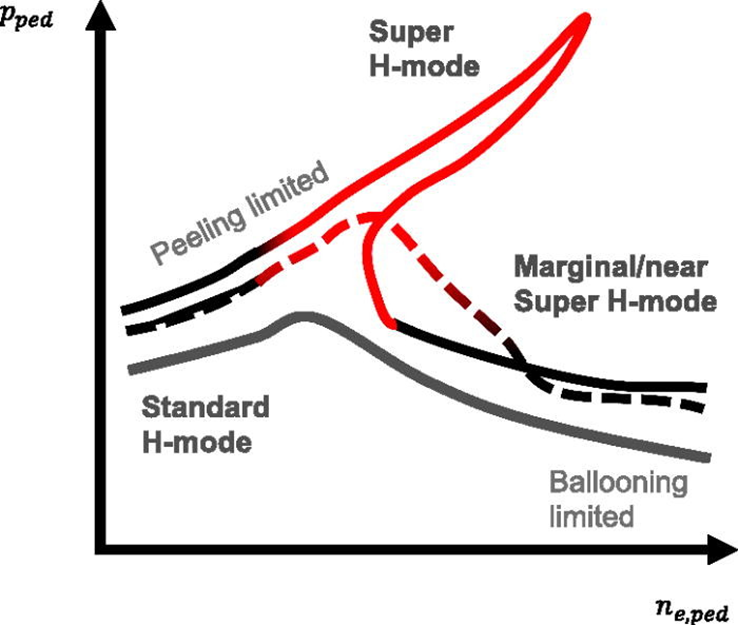
\includegraphics[width=0.45\linewidth]{images/PedBifurcationSuperHmode}
		\label{fig:superhmode}
	} \quad
	\subfloat[Equilibrium configurations and \ac{SOL} flow patterns for (a) standard D-shaped tokamak and (b) negative triangularity snowflake divertor tokamak \cite{Medvedev2015}] {
		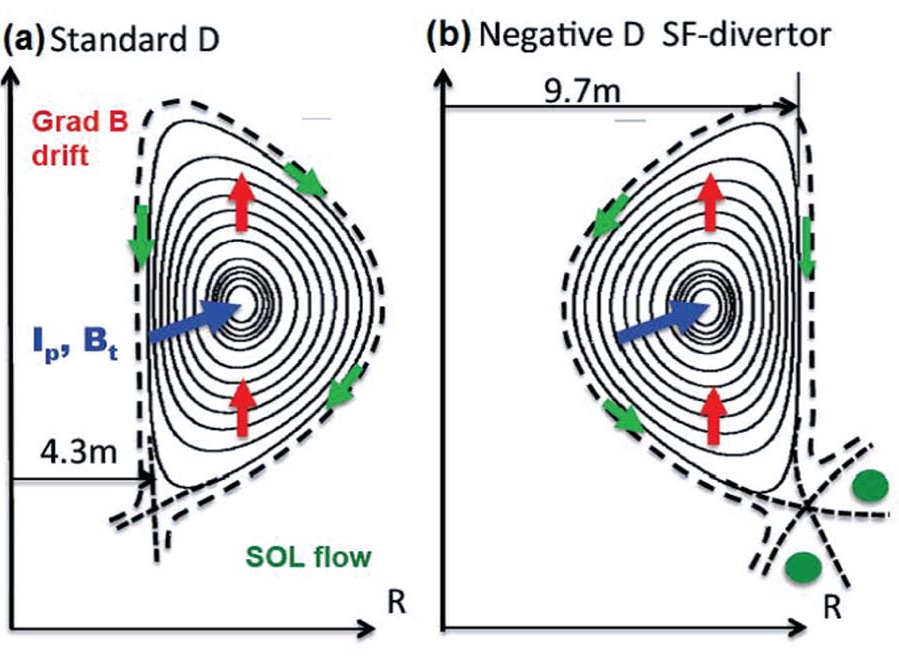
\includegraphics[width=0.5\linewidth]{images/Standard_D_vs_Negative_D}
		\label{fig:standared-d-vs-negative-d}
	}
	\caption{High Performance Operational Regimes}
\end{figure}

Within the plasma community it is known that the exhibited improved performance implies a pinch effect, but a satisfying descriptive model to explain these effects has been elusive. The fluid equations as proposed by \citeauthor{Stacey2017} \cite{Stacey2017} and outlined in \cref{sec:Theory} has the pleasing feature that the long-range \vxb forces are retained in the momentum conservation equations \cref{sub:MomentumConservation} while introducing a more theoretically sound mechanism for particle loss in the form of \ac{IOL}, both thermal and fast. 

The justification that \ac{IOL} is more theoretically sound arises from the observation that diffusion, a near-field effect that is driven by pressure gradients, is an inherently collisional transport mechanism. However, central to the theory of a plasma is that it is most assuredly not. The \ac{IOL} argument is that the particles within a flux surface, to a first order, satisfy conservation canonical angular momentum, energy, and magnetic moment, as will be discussed in \cref{sub:IOL}. The flux surface energy, in the form of temperature, is a Maxwellian distribution, which means particles in the tail, have sufficient energy to take particles beyond the \ac{LCFS}. Both magnetic field irregularities and physical barriers, such as walls, result in particles being removed while trying to execute orbits. 

The inclusion of long-range \vxb forces into the momentum conservation as discussed in \cref{sub:MomentumConservation} is satisfying because it forces the equilibrium solution for the pressure field to re-balance in the presence of the fluid velocities, both the toroidal, $V_\psi$, and poloidal, $V_\theta$.

The fluid theory presented in this paper has developed in some form at the \ac{GIT} \ac{FRC} for as long as fusion has been actively researched there. However, the effort to fully describe the physics in the edge and pedestal region were outlined in \citetitle{Stacey2003}\cite{Stacey2003}.  Stacey and Groebner lay out the physics constraints that are important to an plasma edge/pedestal model in Section II and detail a road-map on the work required realize the ultimate goal stated in Section VI, a fully predictive pedestal model. 

The formal statement of this fluid theory appears first in \citetitle{Stacey2004} from \citeauthor{Stacey2004}\cite{Stacey2004}. Many of the modeling assumptions, such as the observation that a phase space integration of the generalized continuity equation results in only a radially flux or the form of the effective diffusion coefficient, are presented. In a series of several papers, \cite{Stacey2008, Stacey2012, Floyd2012, Wilks2016}, the transport formalism that is being studied in this paper was used to interpret particle flux, \ac{IOL}, and intrinsic rotation based on experimental input of density and temperature. In fact, the model was shown to have an agreement with experimental rotation velocity data from DIII-D to within 10-20\%\cite{Stacey2012}.

The next step, and the objective of this research, is the final step of the 2003 paper \cite{Stacey2003}  is to produce a predictive transport model that conserves particles, momentum and energy by including the non-diffusive loss mechanism of \ac{IOL} and retaining the long range electromagnetic contributions of \vxb. A necessary and intermediate step is to provide an iterative computational algorithm that is compatible with the strong E\&M and \vxb forces simultaneously with the weaker scattering forces. To this end, we will explore the Broyden algorithm, a quasi Newton-Raphson method, as the primary iterative solver in combination with Gauss reduction. A validation exercise against a variety of operational modes, \gls{L-Mode}, \gls{H-Mode}, \gls{NT-Mode}, and \ac{RMP} is envisioned. The result will be a code that predicts the radial density, pressure, and temperature fields as well as the associated toroidal and poloidal velocities.
